%%%%%%%%%%%%%%%%%%%%%%%%%%%%%%%%%%%%%%%%%
%
% (c) 2018 by Jennifer Laaser
%
% This work is licensed under the Creative Commons Attribution-NonCommercial-ShareAlike 4.0 International License. To view a copy of this license, visit http://creativecommons.org/licenses/by-nc-sa/4.0/ or send a letter to Creative Commons, PO Box 1866, Mountain View, CA 94042, USA.
%
% The current source for these materials is accessible on Github: https://github.com/jlaaser/pogil-polymers
%
%%%%%%%%%%%%%%%%%%%%%%%%%%%%%%%%%%%%%%%%%

\renewcommand{\figpath}{content/polymchem/stepgrowth/dispersity/figs}

\begin{activity}[Molecular Weight Distributions in Step-Growth Polymerizations]

\begin{instructornotes}

	This activity introduces students to key concepts related to the molecular weight distributions obtained in step-growth polymerizations.
	
	After completing this activity, students will be able to:
			\begin{enumerate}
				\item ...
			\end{enumerate}
			
	\subsection*{Activity summary:}
	\begin{itemize}
		\item \textbf{Activity type:} Learning Cycle
		\item \textbf{Content goals:} Molecular weight distributions and dispersity in step-growth polymerizations
		\item \textbf{Process goals:} %https://pogil.org/uploads/attachments/cj54b5yts006cklx4hh758htf-process-skills-official-pogil-list-2015-original.pdf
			written communication, critical thinking, information processing
		\item \textbf{Duration:} TBD
		\item \textbf{Instructor preparation required:} none beyond knowledge of relevant content
		\item \textbf{Related textbook chapters:}
			\begin{itemize}
				\item \emph{Polymer Chemistry} (Hiemenz \& Lodge): section 2.4
			\end{itemize}
	\end{itemize}

\end{instructornotes}

	%\textbf{Focus question:} Put a central question for the students to consider through this exercise here.

\begin{model}[Probabilities of Forming Different Chain Lengths]

Suppose we perform a step-growth polymerization of AB-type monomers and stop the polymerization at extent of reaction $p$ (i.e. we stop the polymerization when a fraction $p$ of the A groups have reacted).

Consider the following argument:

\begin{enumerate}
\item For a given AB-type monomer ($i=1$), 
\begin{itemize}
	\item the probability that the A group has \textit{not} reacted, and the monomer stays an AB monomer, is $1-p$, while

	\item the probability that the A group \textit{has} reacted, and has formed at least an AbaB dimer, is $p$.
\end{itemize}

\item Of the dimers ($i=2$),
\begin{itemize}
	\item the probability that the A end group remains unreacted (and the chain stays a dimer) is $1-p$.  Thus if we multiply this probability by the probability of forming a dimer in the first place (which was $p$), the total probability of forming a dimer that stays a dimer is $(1-p)p$, while

	\item the probability that the A end group reacts to form at least a trimer is $p$, so the total probability of forming at least a trimer is $p^2$.
\end{itemize}

\item Of the trimers ($i=3$),
\begin{itemize}
	\item the probability that the A end group remains unreacted is $1-p$.  Thus the total probability of forming a trimer (that stays a trimer) is $(1-p)p^2$, while
	\item the probability that the A end group reacts to form at least a tetramer is $p$, for a total probability of $p^3$.
\end{itemize}
\end{enumerate}

%\vspace{0.1in}
%\centerline{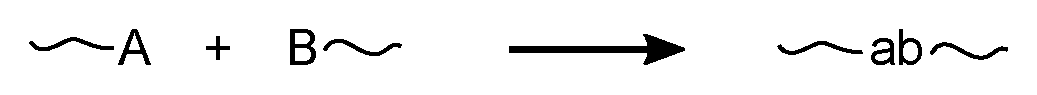
\includegraphics[width=0.6\textwidth]{\figpath/ABrxn.pdf}}

\end{model}

\vspace{0.05in}
\begin{ctqs}

	\question What is the probability of forming a tetramer ($i=4$) that stays a tetramer?
	
	\question What is the probability of forming at least a pentamer ($i=5$)?
	
	\question Fill in the following table:
	
		\begin{center}
			\renewcommand{\arraystretch}{4}
			\begin{tabular}{|c|c|}
				\hline
				\textbf{~~i~~} & {\renewcommand{\arraystretch}{1}\begin{tabular}{c}\textbf{Probability of forming a chain of length $i$}\\\textbf{that does not grow any longer}\end{tabular} }\\\hline
				1 & \\\hline
				2 & \\\hline
				3 & \\\hline
				4 & \\\hline
				5 & \\\hline
			\end{tabular}
		\end{center}
	
	\question What pattern do you notice in these values?
	
	\question Complete the following statement:
	
		``The probability of forming an i-mer that stays an i-mer is \line(1,0){50}.''
		
\end{ctqs}

\begin{infobox}

	The probability of making an i-mer that stays an i-mer is the same as the probability of a given chain being an i-mer, because the number of chains of length $i$ is directly proportional to the probability of making a chain of length $i$.
	
	As a consequence, the mole fraction of chains with length $i$, $x_i$, is equal to the probability of making an i-mer that stays an i-mer.

\end{infobox}

\begin{ctqs}
	\question \label{stepdispersity:ctq:xi} W What is the mole fraction of chains with length $i$?
	
	\question Calculate the mole fractions of chains with length $i$ for $p=0.5$ and $p=0.9$, and use your results to fill in the following table:
	
		\begin{center}
			\renewcommand{\arraystretch}{4}
			\begin{tabular}{|c|c|c|}
				\hline
				\textbf{~~$i$~~} & $x_i$ when $p=0.5$ & $x_i$ when $p=0.9$ \\\hline
				1 & & \\\hline
				2 & & \\\hline
				3 & & \\\hline
				5 & & \\\hline
				10 & & \\\hline
				15 & & \\\hline
				20 & & \\\hline
			\end{tabular}
		\end{center}
		
	\question Plot your results on the following axes.  Make sure to use a different symbol for points corresponding to $p=0.5$ than for the points corresponding to $p=0.9$.
	
	\question How are the plots for $p=0.5$ and $p=0.9$ similar, and how are they different?  Briefly describe your observations in 2-3 complete sentences.
	
	\question \label{stepdispersity:ctq:xiplus1} What is the mole fraction of chains with length $i+1$?
	
	\question Compare your answer to question \ref{stepdispersity:ctq:xiplus1} with that to question \ref{stepdispersity:ctq:xi}. Can the mole fraction of chains with length $i+1$ ever be \emph{greater} than the mole fraction of chains with length $i$?  Justify your answer in 1-2 complete sentences.
	
	\question Comment briefly on whether or not your answer to the preceding question is consistent with your plots.
	
\end{ctqs}


\begin{model}[$M_n$ and $M_w$]

Sdf

\end{model}

\begin{ctqs}
		\question sdf
			
\end{ctqs}

\begin{exercises}

		\exercise sdf
\end{exercises}
	
\end{activity}